\documentclass[tikz,border=5pt]{standalone}

\usepackage{fontspec}
\usepackage{unicode-math}
\usepackage{pgfplots}
\usepgfplotslibrary{groupplots}

\pgfplotsset{compat=1.18}

% Compile with LuaLaTeX or XeLaTeX.
\setmainfont{STIX Two Text}
\setmathfont{STIX Two Math}

\colorlet{rulecolor}{blue!65!black}

\begin{document}

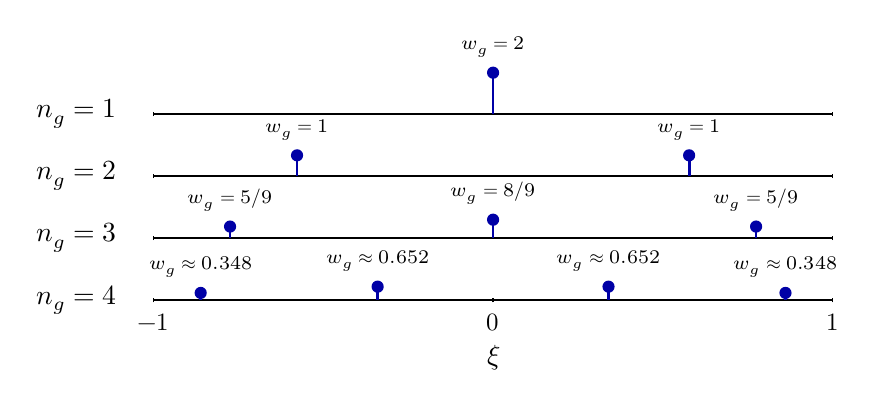
\begin{tikzpicture}

  \begin{groupplot}[
      group style={
          group size=1 by 4,
          vertical sep=0.12cm,
        },
      width=11.5cm,
      height=2.25cm,
      xmin=-1.22, xmax=1.08,
      ymin=-0.28, ymax=2.28,
      axis lines=none,
      clip=false,
    ]

    % n_g = 1
    \nextgroupplot
    \node[anchor=east, font=\normalsize] at (axis cs:-1.08,0) {\(n_g=1\)};
    \draw[black, semithick] (axis cs:-1,0) -- (axis cs:1,0);
    \draw[black, semithick] (axis cs:-1,-0.11) -- (axis cs:-1,0.11);
    \draw[black, semithick] (axis cs:1,-0.11) -- (axis cs:1,0.11);
    \draw[rulecolor, line width=1pt] (axis cs:0,0) -- (axis cs:0,2);
    \fill[rulecolor] (axis cs:0,2) circle (2.2pt)
      node[above=2pt, black, font=\scriptsize] {\(w_g=2\)};

    % n_g = 2
    \nextgroupplot
    \node[anchor=east, font=\normalsize] at (axis cs:-1.08,0) {\(n_g=2\)};
    \draw[black, semithick] (axis cs:-1,0) -- (axis cs:1,0);
    \draw[black, semithick] (axis cs:-1,-0.11) -- (axis cs:-1,0.11);
    \draw[black, semithick] (axis cs:1,-0.11) -- (axis cs:1,0.11);
    \draw[rulecolor, line width=1pt]
    (axis cs:-0.577350,0) -- (axis cs:-0.577350,1);
    \draw[rulecolor, line width=1pt]
    (axis cs:0.577350,0) -- (axis cs:0.577350,1);
    \fill[rulecolor] (axis cs:-0.577350,1) circle (2.2pt)
      node[above=2pt, black, font=\scriptsize] {\(w_g=1\)};
    \fill[rulecolor] (axis cs:0.577350,1) circle (2.2pt)
      node[above=2pt, black, font=\scriptsize] {\(w_g=1\)};

    % n_g = 3
    \nextgroupplot
    \node[anchor=east, font=\normalsize] at (axis cs:-1.08,0) {\(n_g=3\)};
    \draw[black, semithick] (axis cs:-1,0) -- (axis cs:1,0);
    \draw[black, semithick] (axis cs:-1,-0.11) -- (axis cs:-1,0.11);
    \draw[black, semithick] (axis cs:1,-0.11) -- (axis cs:1,0.11);
    \draw[rulecolor, line width=1pt]
    (axis cs:-0.774597,0) -- (axis cs:-0.774597,0.555556);
    \draw[rulecolor, line width=1pt]
    (axis cs:0,0) -- (axis cs:0,0.888889);
    \draw[rulecolor, line width=1pt]
    (axis cs:0.774597,0) -- (axis cs:0.774597,0.555556);
    \fill[rulecolor] (axis cs:-0.774597,0.555556) circle (2.2pt)
      node[above=2pt, black, font=\scriptsize] {\(w_g=5/9\)};
    \fill[rulecolor] (axis cs:0,0.888889) circle (2.2pt)
      node[above=2pt, black, font=\scriptsize] {\(w_g=8/9\)};
    \fill[rulecolor] (axis cs:0.774597,0.555556) circle (2.2pt)
      node[above=2pt, black, font=\scriptsize] {\(w_g=5/9\)};

    % n_g = 4
    \nextgroupplot
    \node[anchor=east, font=\normalsize] at (axis cs:-1.08,0) {\(n_g=4\)};
    \draw[black, semithick] (axis cs:-1,0) -- (axis cs:1,0);
    \draw[black, semithick] (axis cs:-1,-0.11) -- (axis cs:-1,0.11);
    \draw[black, semithick] (axis cs:0,-0.11) -- (axis cs:0,0.11);
    \draw[black, semithick] (axis cs:1,-0.11) -- (axis cs:1,0.11);
    \draw[rulecolor, line width=1pt]
    (axis cs:-0.861136,0) -- (axis cs:-0.861136,0.347855);
    \draw[rulecolor, line width=1pt]
    (axis cs:-0.339981,0) -- (axis cs:-0.339981,0.652145);
    \draw[rulecolor, line width=1pt]
    (axis cs:0.339981,0) -- (axis cs:0.339981,0.652145);
    \draw[rulecolor, line width=1pt]
    (axis cs:0.861136,0) -- (axis cs:0.861136,0.347855);
    \fill[rulecolor] (axis cs:-0.861136,0.347855) circle (2.2pt)
      node[above=2pt, black, font=\scriptsize] {\(w_g\approx0.348\)};
    \fill[rulecolor] (axis cs:-0.339981,0.652145) circle (2.2pt)
      node[above=2pt, black, font=\scriptsize] {\(w_g\approx0.652\)};
    \fill[rulecolor] (axis cs:0.339981,0.652145) circle (2.2pt)
      node[above=2pt, black, font=\scriptsize] {\(w_g\approx0.652\)};
    \fill[rulecolor] (axis cs:0.861136,0.347855) circle (2.2pt)
      node[above=2pt, black, font=\scriptsize] {\(w_g\approx0.348\)};

    \node[anchor=north, font=\small] at (axis cs:-1,-0.18) {\(-1\)};
    \node[anchor=north, font=\small] at (axis cs:0,-0.18) {\(0\)};
    \node[anchor=north, font=\small] at (axis cs:1,-0.18) {\(1\)};
    \node[anchor=north, font=\normalsize] at (axis cs:0,-1.7) {\(\xi\)};

  \end{groupplot}

\end{tikzpicture}

\end{document}
